\documentclass{sigchi}

% Remove or comment out these two lines for final version
\toappearbox{\Large Submitted to IUI'14. \\Do not cite, do not circulate.}
\pagenumbering{arabic}% Arabic page numbers for submission. 

% Use \toappear{...} to override the default ACM copyright statement (e.g. for preprints).

% Load basic packages
\usepackage{balance}  % to better equalize the last page
\usepackage{graphics} % for EPS, load graphicx instead
\usepackage{times}    % comment if you want LaTeX's default font
\usepackage{url}      % llt: nicely formatted URLs
\usepackage{amssymb}
\usepackage{amsmath}

\usepackage{caption}
\usepackage{subcaption} 
\DeclareCaptionType{copyrightbox}


% llt: Define a global style for URLs, rather that the default one
\makeatletter
\def\url@leostyle{%
  \@ifundefined{selectfont}{\def\UrlFont{\sf}}{\def\UrlFont{\small\bf\ttfamily}}}
\makeatother
\urlstyle{leo}


% To make various LaTeX processors do the right thing with page size.
\def\pprw{8.5in}
\def\pprh{11in}
\special{papersize=\pprw,\pprh}
\setlength{\paperwidth}{\pprw}
\setlength{\paperheight}{\pprh}
\setlength{\pdfpagewidth}{\pprw}
\setlength{\pdfpageheight}{\pprh}

% Make sure hyperref comes last of your loaded packages, 
% to give it a fighting chance of not being over-written, 
% since its job is to redefine many LaTeX commands.
\usepackage[pdftex]{hyperref}
\hypersetup{
pdftitle={SIGCHI Conference Proceedings Format},
pdfauthor={LaTeX},
pdfkeywords={SIGCHI, proceedings, archival format},
bookmarksnumbered,
pdfstartview={FitH},
colorlinks,
citecolor=black,
filecolor=black,
linkcolor=black,
urlcolor=black,
breaklinks=true,
}


% create a shortcut to typeset table headings
\newcommand\tabhead[1]{\small\textbf{#1}}


% End of preamble. Here it comes the document.
\begin{document}

\title{Investigating Co-adaptation in a Handwriting Recognition System}

% Note that submissions are blind, so author information should be omitted
\numberofauthors{3}
\author{
  \alignauthor 1st Author Name\\
    \affaddr{Affiliation}\\
    \affaddr{Address}\\
    \email{e-mail address}\\
    \affaddr{Optional phone number}
  \alignauthor 2nd Author Name\\
    \affaddr{Affiliation}\\
    \affaddr{Address}\\
    \email{e-mail address}\\
    \affaddr{Optional phone number}    
  \alignauthor 3rd Author Name\\
    \affaddr{Affiliation}\\
    \affaddr{Address}\\
    \email{e-mail address}\\
    \affaddr{Optional phone number}
}

% Teaser figure can go here
%\teaser{
%  \centering
%  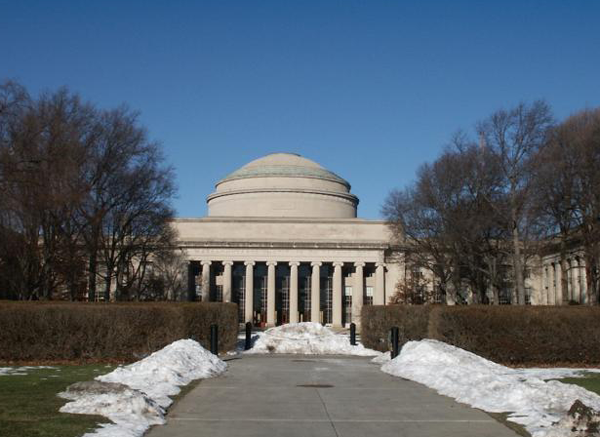
\includegraphics{Figure1}
%  \caption{Teaser Image}
%  \label{fig:teaser}
%}

\maketitle

\begin{abstract}
Handwriting recognition is a natural and versatile method for data
entry, especially on mobile devices and devices with touch
screens. However, as handwriting is highly variable, it is difficult
to design handwriting recognizers that perform well for everyone. A
natural solution is to use machine learning to adapt the recognizer to
the user. One complicating factor is that, as the computer is adapting
to the user, the user is also adapting to the computer. The
contributions of this paper are in three complementary
directions. First, we devise an information-theoretic framework for
quantifying the efficiency of a handwriting system where the system
includes both the user and the computer. From this framework, we
derive two performance measures that are used to gamify handwriting
adaptation. Second, we develop and deploy an adaptive handwriting
recognition system in the context of a game that runs on iOS
devices. Finally, we perform a statistical analysis of the system’s
performance on the data collected from 15 different users over
multiple sessions and characterize the impact of machine adaptation
and of human adaptation.
\end{abstract}

\keywords{
  Co-adaptation; handwriting recognition; communication channel;
%  Guides; instructions; author's kit; conference publications;
%  keywords should be separated by a semi-colon.
%	\\\textcolor{red}{Mandatory section to be included in your final version.}
}

\category{H.5.2}{Information Interfaces and Presentation (e.g. HCI)}{User Interfaces
%\\
%\textcolor{red}{See: \url{http://www.acm.org/about/class/1998/}
%for more information and the full list of ACM classifiers and descriptors. 
%Mandatory section: On the submission page
%only the classifiers' letter-number combination will need to be entered.}
}

\terms{
	Algorithms; Measurement; Human Factors
%	If you choose more than one ACM General Term, 
%	separate the terms with a semi-colon.
%\\
%\textcolor{red}{If you choose more than one ACM General Term, 
%separate the terms with a semi-colon. See list of ACM terms at:
%\url{http://www.sheridanprinting.com/sigchi/generalterms.htm}.
%Optional section to be included in your final version.}
}

\newtheorem{theorem}{Theorem}   
\newtheorem{lemma}[theorem]{Lemma}

\section{Introduction}

One of the challenges brought on by the miniaturization of mobile
computing devices such as smart phones and tablets is the difficulty of
entering information into the device. The communication bandwidth from
the device to the human, utilizing high-resolution screens and high
fidelity sound, is very high. However, the bandwidth from the human to
the device is severely constrained by the size of our fingers and by
the difficulty of performing voice recognition in noisy environments.

As the screen real estate becomes scarce, the standard soft-keyboard
can only fit up to about 40 fingertip-sized keys on one screen. While
40 keys are sufficient for languages with a small set of characters
such as English, it is not suitable for languages with more characters
such as Thai or Chinese which contains more than 60 and thousands of
different characters respectively. For such languages, as well as in
the multilingual settings, the users are required to either repeatedly
switch between different keyboard layouts in order to find the desired
character.

\newcommand{\tm}{\textsuperscript{\textregistered}~}

Many alternatives to the standard soft-keyboard exist. For example,
Swype\tm provides a method for tracing a path between keyboard keys
and lifting the finger from the screen at the end of each
word. Dasher~\cite{Garrett2003} is a particularly innovative method
where typing is replaced by using a joystick-like pointer to fly
through clouds of characters. Finally, there are handwriting
recognition software that allow the user to enter information using
natural handwriting.

A user of any one of these methods typically improves significantly
with practice. There are many competitions between different data
entry methods. However, these comparisons are inherently flawed in
that the contender is always a person who can enter information faster
than the current record holder, most likely as a result of extensive
training. In other words, {\em user adaptation} cannot be ignored.

To evaluate the efficiency of a particular data entry method, it is
therefore necessary to measure the performance of each user over a
sufficiently long period of time so that the performance of the user
stabilizes. As we are interested in machine learning methods, we arrive
at the interesting situation in which both the computer and the human
adapt over time in an effort to maximize the input rate of the
data entry method. We refer to this situation as {\em co-adaptation}.

Designing an intelligent system that co-adapts with the users is a
challenging problem on its own~\cite{Hook2000, Maes1994, Lim2009a}.
Our goal in this paper is not to address those challenges, but rather
to focus on characterizing the impact of machine adaptation and of
human adaptation in the context of handwriting recognition.
 
The paper is organized as follows. First, we propose an
information-theoretic framework for quantifying the efficiency of a
handwriting system where the system includes both the user and the
computer. Next, we describe our adaptive handwriting recognition
algorithm that we developed for our experiment. Then, we describe the
experiment and present the results in terms of the performance
measures derived from the proposed framework Finally, we draw some
conclusions.


\section{Handwriting recognition as a communication channel}
\label{sec:channel}

Unlike typing, which transmits information to the computer at discrete
time points, handwriting continuously transmits information as the
writer creates the trajectory. Traditionally, handwriting data is
analyzed one ``unit'' at a time where ``unit'' can be a stroke, a
chracter, a word or even a sentence. In this work, we propose an
alternative analysis where the data is analyzed in fixed intervals of
time. We consider the process of writing as a process through which
the intended letter is disambiguated from the other possible letters.

% input
\newcommand{\intent}{M}
\newcommand{\intentSet}{\mathcal{E}}
\newcommand{\intentDist}{\mathcal{M}}
% output
\newcommand{\pred}[1]{\mathcal{Q}_{#1}}
\newcommand{\predFinal}{\pred{\mathrm{final}}}
% trajectory
\newcommand{\writing}[1]{W_{1:{#1}}}
\newcommand{\writingVec}{\overline{W}}
\newcommand{\writingDist}{P(\writingVec | \intent)}
% misc
\newcommand{\tFinal}{T}
\newcommand{\expectedDuration}{\mathbb{E} \left[\tFinal\right]}
\newcommand{\condEntropy}{H(\predFinal | \intent)}

We formalize this process using the concept of a communication
channel~\cite{Shannon1948}.  Let $\intentSet$ denote the set of all
possible input. Technically, $\intentSet$ can be a set of sentences, a
set of words, or a set of characters. Without loss of generality, in
this work, we assume that $\intentSet$ is a set of 26 English
characters. We also ignore dependencies between characters due to
the language model and due to the co-articulation effects between
neighboring handwritten characters.

As shown in Figure~\ref{fig:hwr_channel}, the channel is comprised of
two separate processes. First, the handwriting process is the process
of which the user translates an intent $\intent \in \intentSet$ into a
series of hand movements which is sampled at some rate to create a
discrete time trajectory: $\writing{T} = \left[ (x_1,y_1), \ldots,
  (x_T,y_T) \right]$. In other words, this process {\em encodes} the
intent $\intent$ into a trajectory $\writing{T}$. The distribution
$\writingDist$ denotes the variability of the encoding process. The
second process is the recongition process that decodes the handwriting
trajectory into the original intent. For each time step $1 \le t \le
T$, the process maps a trajectory $\writing{t}$ to a distribution over
$\intentSet$, denoted by $\pred{t}$.

\begin{figure}
  \centering
  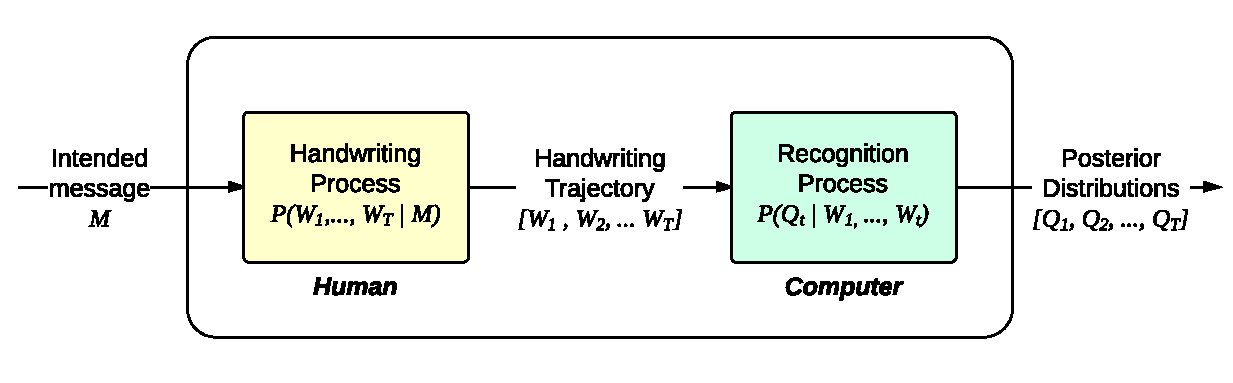
\includegraphics[width=0.9\columnwidth]{figures/hwr_channel.pdf}
  \caption{A summary of the handwriting recognition channel.}
  \label{fig:hwr_channel}
\end{figure}

Let $\tFinal$ and $\predFinal$ denote the time and the posterior
distribution when the user finishes writing the trajectory
respectively.  According to the theory of channel capacity, the
information transmitted through the channel is quantified by the
mutual information between the input $\intent$ and the decoding
posterior $\predFinal$, denoted by $I(\intent ; \predFinal)$. We
define the mean posterior of $\predFinal$ conditioned on $\intent$ and
the average posterior distribution as follows.
\[
P(\predFinal | \intent) =
\int\limits_{\writingVec \sim \writingDist} { P(\predFinal | \writingVec)
P(\writingVec | \intent)} 
\]
\[
P(\predFinal)
=
\sum_{m \in \intentSet} 
P(\intent = m) P(\predFinal | \intent = m)
\]
Given these two expressions, we can define the mutual information
between the character $\intent$ and the decoding $\predFinal$ to be 
{
\small
\[
I(\intent ; \predFinal) = 
H(\predFinal)
- \sum_{m \in \intentSet} P(\intent = m) H(\predFinal | \intent = m)
\]

}
where the entropy of $\predFinal$ is defined as
\[
H(\predFinal) = -\sum_{m \in \intentSet} {
P(\predFinal = m) \log_2 P(\predFinal = m)}
\]

\newcommand{\RMI}{R_{\mathrm{MI}}}
\newcommand{\RLL}{R_{\mathrm{LL}}}

Now we define the channel rate to be 
\begin{align}
\label{eq:channel_rate}
\RMI
= 
\frac{I( \intent ;  \predFinal)}{\expectedDuration}
\end{align}

The channel rate $\RMI$ is not suitable for practical implementation
for two reasons. First, the estimates of $\RMI$ relies on the
estimates of $H(\predFinal | \intent)$ which typically require an
extensive amount of data. Secondly, suppose the original intent is
$m$, $\RMI$ yeilds a high value as long as $P(\predFinal | \intent =
m)$ concentrates on some intent $n$ regardless of whether $n = m$.  We
propose an alternative to the $\RMI$, called $\RLL$, based on the idea
of log loss. We define $\RLL$ to be
{ 
\scriptsize
\begin{align}
\label{eq:channel_rate_ll}
\RLL = \frac{H(\predFinal) 
 - \displaystyle\sum_{m \in \intentSet} P(\intent = m) (-\log_2 P(\predFinal = m | \intent = m))}{\expectedDuration}
\end{align}
}

\begin{lemma}
\label{lemma:bound}
Let $P_{i,j}$ denote $P(\predFinal = i | \intent = j)$. For any intent $m \in \intentSet$ and $a = -\log_2 P_{m,m}$, then 
\[ H(\predFinal | \intent=m) \leq a + a^{-1} + \log_2
(|\intentSet|-1) \]
\end{lemma}
\begin{proof}
By definition:
\[ H(\predFinal | \intent=m) = -\displaystyle\sum_{i \in \intentSet} P_{i,m} \log P_{i,m}\]
Given the value of $P_{i,m}$, the entropy is maximized if the
remaining probability is divided uniformly across the remaining $|\intentSet|-1$
values. Let $p$ denote $P_{m,m}$.
\[
 H(\predFinal | \intent=m) \leq -p \log_2 p - (1-p) \log_2 \left(\frac{1-p}{|\intentSet|-1}\right)
\]
We can rewrite this expression as 
{
\small
\[
 H(\predFinal | \intent=m) \leq -p \log_2 p - (1-p) \log_2 (1-p) +
 (1-p) \log_2 (|\intentSet|-1)
\]
}
Using the definition $a = -\log_2 p$, we have $p = 2^{-a}$. We can
bound each term on the right hand side as follows. 
\[
 H(\predFinal | \intent=m) \leq a + a^{-1} + \log_2 (|\intentSet|-1)
\]
\end{proof}

From Lemma~\ref{lemma:bound}, it follows that when $-\log_2
P(\predFinal = m | \intent = m)$ is small then the conditional entropy
$H(\predFinal | \intent)$ is also small. As a result, the mutual
information $I( \intent ; \predFinal)$ will be close to its maximal
possible value of $H(\predFinal)$. In other words, the log loss
$-\log_2 P(\predFinal = m | \intent = m)$ provides an upper bound for
the conditional entropy $H(\predFinal | \intent)$.

Intuitively, the channel rate is a measure that quantifies both
accuracy and speed of a handwriting recognition channel at the same
time. Handwriting, as well as many other motor control tasks, obeys
the speed-accuracy tradeoff~\cite{Fitts1954}. It is not sufficient to
quantify the efficiency of a handwriting recognition system by its
recognition accuracy alone. For example, a system that requires the
user to write each character in a specialized form may attain a very
high recognition accuracy, but it would require the user more time and
effort to use. Such system might not be as efficient as a system that
makes more errors but allows the user to write freely. In a sense,
maximizing the channel rate is equivalent to finding a balance between
maximizing the recognition accuracy and minimizing the writing time
and effort of the user.

Based on this framework, we suggest that the channel rate can be improved
by a combination of human learning and machine learning, which
corresponds to improving the handwriting process and the recognition
process respectively. Ideally, $\predFinal$ is always concentrated
on the original intent $\intent$. This would mean that the channel is
perfect and works without error. However, in real-world scenarios,
errors will occur. One source of errors comes from misrecognition in
the recognition process. These recognition errors can be reduced using
training data and machine learning. The harder problem is when there
is a significant overlap between $\writingDist$ for different
intents. In this situation, we need to rely on the user to make
their handwriting less ambiguous. Although the effect of human
learning is always present, we believe that it can be enhanced by
giving useful feedback to the user in the form of guidance or lessons.


\section{Adaptive recognition algorithm}
\label{sec:recognition_algorithm}

\newcommand{\prototypeSet}{\mathcal{P}}

We developed an adaptive handwriting recognition algorithm that maps a
handwriting trajectory $\writing{t}$ to a posterior distribution over
$\intentSet$, denoted by $\predFinal$. By realizing that the effect of
user adaptation is likely to be present, we designed our recognition
algorithm so that it can adapt not only to each individual user, but
also to the changes of the handwriting trajectory distribution
$\writingDist$ unique to each user over time. The idea of specializing
and adapting the recognizer for each user has been studied and shown
to be effective in reducing the error rate~\cite{Connell2002, Matic93,
  Kienzle06}.

At a high-level, our adaptive recognition system can be outlined as
follows. For each user, the system creates and maintains one or more
Markov-based models~\cite{ThomasPloetz2011} for each element in
$\intentSet$. We refer to each of such models as a {\em
  prototype}. Each prototype is a left-to-right HMM with Gaussian
observations with each of the hidden states correponds to a sample
point in the trajectory. Let $\prototypeSet_u$ denote a set of
prototypes for a user $u$. The adaptivity of our system comes from the
re-training of $\prototypeSet_u$. In decoding, given a handwriting
trajectory and a set of prototypes $\prototypeSet_u$, the system
computes a posteior distribution $\predFinal$ and, when a single
prediction is needed, the element with the maximum likelihood is
predicted.

\subsection{Feature vectors and distance function}

As a preprocessing step, each instance of the handwriting trajectory
is appended with the supplemental information. After
preprocessing, a handwriting instance is described by a sequence of
feature vectors $\langle f_1, \ldots, f_T \rangle$ where
$f_i = (x_i,y_i, dx_i,dy_i)$. $(x_i,y_i)$ denotes the normalized
touchscreen coordinate and $(dx_i,dy_i) = (\frac{x_i - x_{i-1}}{z},
\frac{y_i - y_{i-1}}{z}) , z = \sqrt{(x_i - x_{i-1})^2 + (y_i -
  y_{i-1})^2}$ denotes the writing direction.

For measuring the similarity between two handwriting instances or a
handwriting instance and a prototype, we use {\it dynamic time
  warping} (DTW) distance~\cite{Rabiner1993} as the distance function
in our algorithm. The DTW distance is commonly used for
variable-length data such as handwriting and speech.

\subsection{Initial adaptation}

The initial adaptation is critical for any intelligent system. It is
unquestionable that the performance of any well-behaved
intelligent system increases as the system learns more about the
user. Many times, the users can get frustrated with the system and stop
using it before it can fully adapt to the user.
 
We address the problem of initial adaptation by leveraging the power
of {\em the crowd}. Typically, people do have similar handwriting
particularly when they share the same educational culture. In the very
first interaction with the user $u$, our system has no information
about the user and, therefore, assign a set of typical prototypes
which has been trained using data from multiple users in the past.  We
refer to this set of prototypes as $\prototypeSet_0$. After the first
interaction, the system selects a set of prototypes
$\prototypeSet_{(u,1)}$ from the database of all prototypes across
different users such that each prototype in the set minimizes the
distance to the corresponding handwriting instances.


\subsection{Adapting the prototypes over time}

After the initial adaptation phase and after the user has given a few
examples of his/her handwriting, the system performs a weighted cluster
analysis using K-means on the data and the current prototypes in
$\prototypeSet_{(u,i)}$ to generate a new set of prototypes
$\prototypeSet_{(u,i+1)}$ such that the new set of prototypes minimizes the
average inter-example distances of the same label. 

Sometimes, a trained prototype has too many hidden states than
necessary. The system performs an additional step to reduce the number
of hidden states by a series of removing and merging hidden states
while maintaining the same recognition power, using a variant of
forward-backward algorithm. Figure~\ref{fig:state_reduction} shows the
hidden states before and after the reduction step.

\begin{figure}
  \centering
  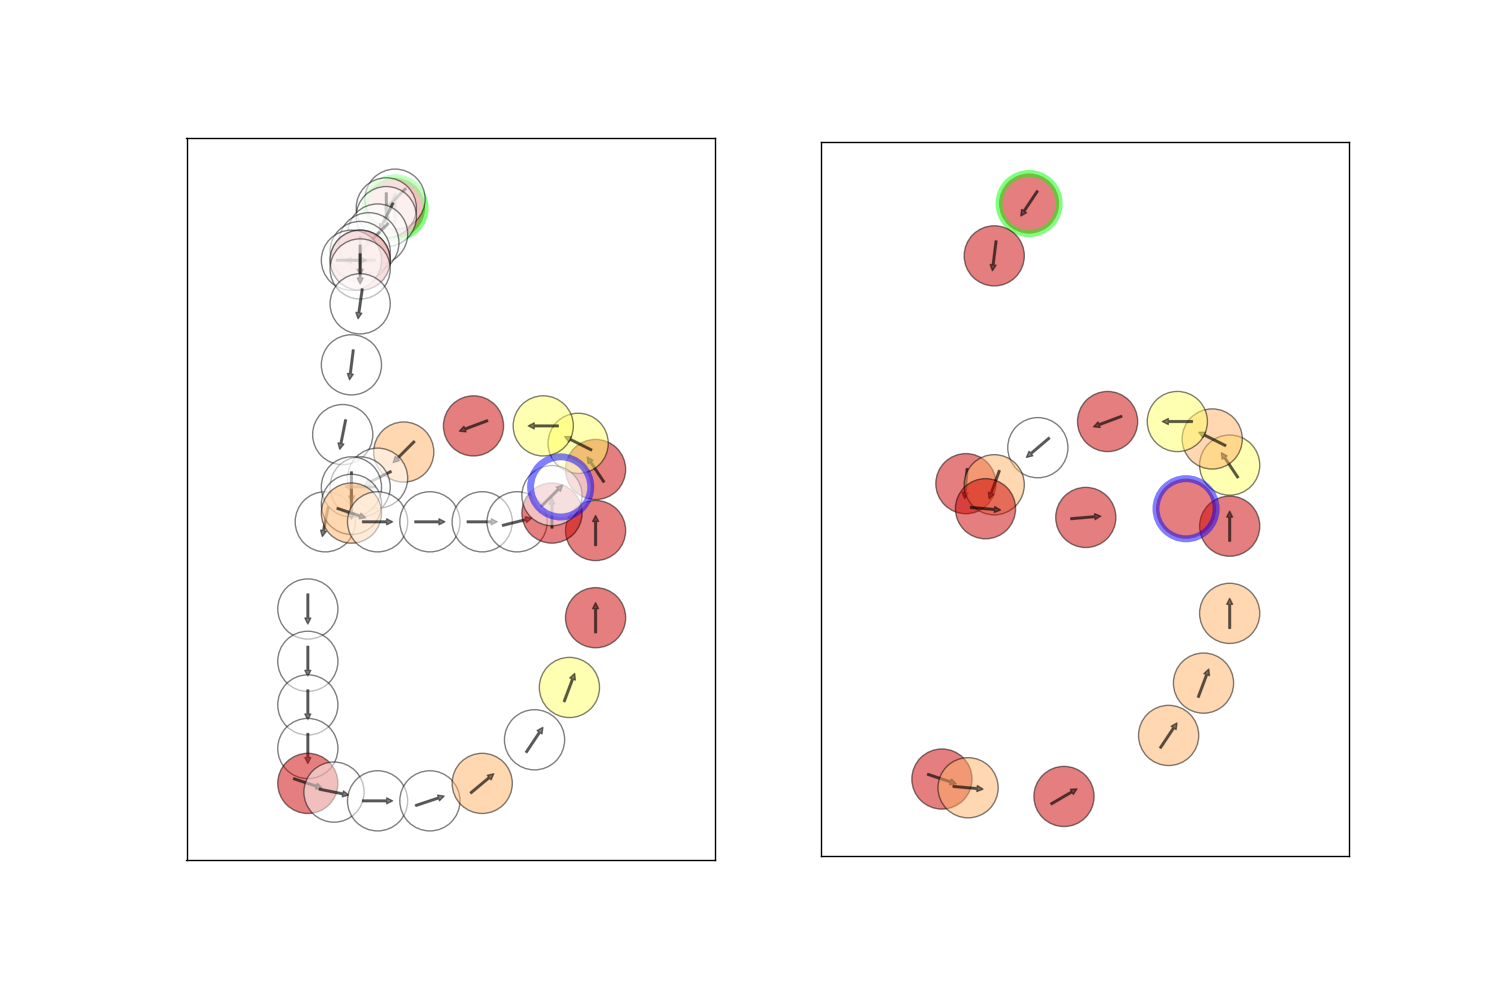
\includegraphics[width=0.9\columnwidth] {figures/state_reduction.png}
  \caption{The hidden state reduction process is applied to each
    prototype to remove rarely visited states with respect to the
    training set. The originally trained prototype is shown on the
    left and the reduced prototype is shown on the right. The
    intensity of the colors corresponds to the expected number of
    times the state being mapped to. }
  \label{fig:state_reduction}
\end{figure}

\subsection{Decoding}

Our decoding algorithm is based on the standard Bayesian inference.
Given a handwriting trajectory $\writing{T}$ and the current set of
prototypes $\prototypeSet_u$, at every time step $1 \le t \le T$, the
algorithm computes the distance from $\writing{t}$ to each of the
prototypes in $\prototypeSet_u$. The distances are transformed into a
probability distribution $\pred{t}$. This decoding process is
implemented using a dynamic programming technique which is similar in
spirit to the forward algorithm~\cite{Bilmes97}. When a single prediction is expected,
the algorithm returns the prediction with the maximum likelihood.


\section{Experiment}
\label{sec:experiment}

\newcommand{\RAdapt}{R_{\mathrm{adapt}}}
\newcommand{\RFixed}{R_{\mathrm{fixed}}}
\newcommand{\RIdeal}{R_{\mathrm{ideal}}}

The main objective of our experiment is to determine and quantify the
effect of machine adaptation and of human adaptation when the users
interact with the system over some period of time.  We conducted an
experiment in the format of a game where the participants were asked
to compete in a writing game. In each session, each participant was
presented with a random permutation of the 26 lowercase English
alphabets i.e. $\intentSet = \left[ a \ldots z \right]$ and
$P(\intent)$ is uniform. The objective of the game was to write the
presented characters as quickly as possible and, more importantly, the
handwritten characters should be recognizable by the system. A score,
which is the average {\it channel rate} of the session, was given to
the user right after each session to reflect the performance of the
session. There were 15 participants in this experiment. We did not
control past experience of the participants. Some of them had more
experience with touch screens than others. Each participant was asked
to play the writing game, which is an implementation our adaptive
recognition algorithm on the Apple iPads and iPhones, for at least 20
sessions over multiple days in his/her own pace.

The experiment was set up to demonstrate a condition called {\em
  co-adaptation} where both the user and the computer were allowed to
adapt together. We denote this condition $\RAdapt$. To investigate the
effect of co-adaptation, we create a controlled condition called
$\RFixed$ where the computer was not allowed to adapt with the
user. In other words, we ran a simulation to figure out what the
channel rates would have been if the prototype sets were never changed
from $\prototypeSet_0$. Ideally, it would be more preferable to have
$\RFixed$ determined by another control group where the prototypes
were kept fixed and never changed. Unfortunately, we found that hard to
do since the experiment was done on volunteers. However, the results
from the simulated condition can be seen as a lower bound on the
amount of the improvement attributable to human learning and, therefore,
it is sufficient to demonstrate our point.


\section{Results and discussion}
\label{sec-results}

The average channel rates per session of the two conditions $\RAdapt$
and $\RFixed$ are shown in Figure~\ref{fig:channel_rate_adapt} and
Figure~\ref{fig:channel_rate_fixed} respectively.

Although the prototype set was not changing in $\RFixed$, we observe
that channel rate increases over the sessions. The paired t-test
indicates a significant difference between the average channel rate in
the first 5 sessions and the average channel rate in the last 5
sessions ($p < 0.0011$). This suggests that the users improve the
handwriting on their own. We call this effect {\em user
  adaptation}.

Figure~\ref{fig:duration} and Figure~\ref{fig:mutual_information}
reveal that the major contribution of {\em user adaptation} comes from
the fact that the users write faster in the last 5 sessions
compared to the first 5 sessions ($p < 0.0001$), and not because of the
system recieved more information from the user ($p = 0.9723$). This
result is as expected according to the law of practice~\cite{Newell1981}.

\begin{figure}
  \centering
  \begin{subfigure}[b]{\columnwidth}
    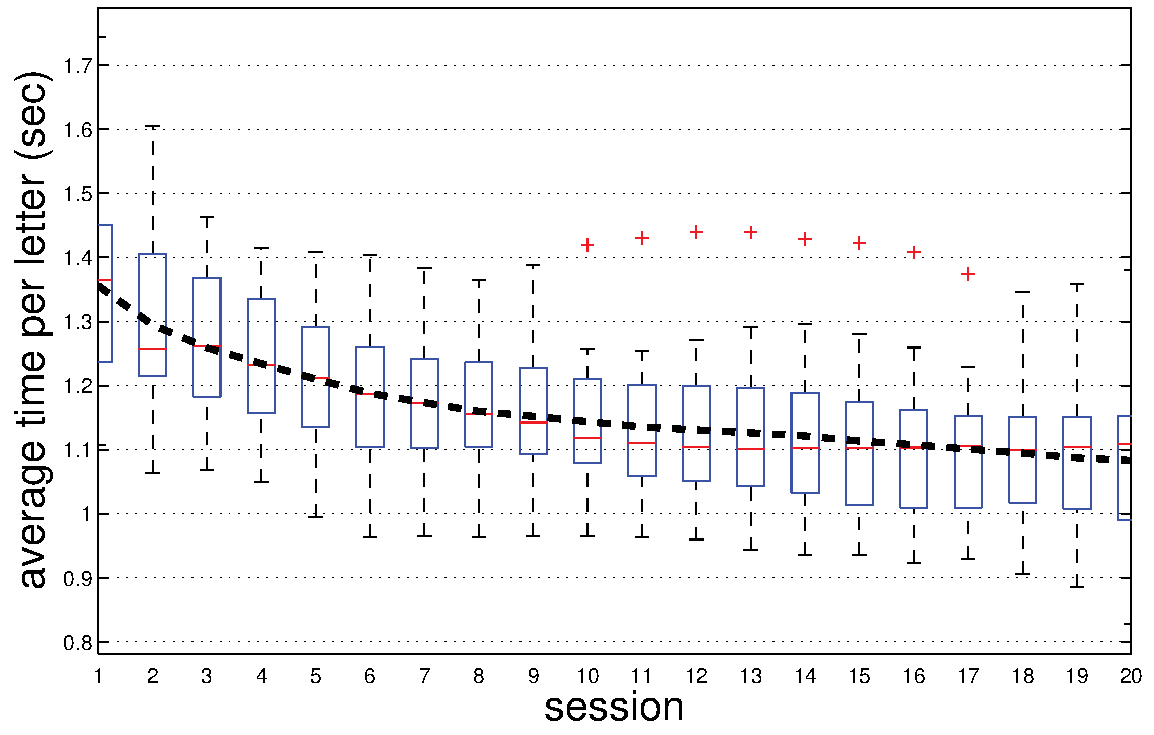
\includegraphics[width=\columnwidth]{figures/IUI_duration_p_adapt.pdf}
    \caption{Writing duration}
    \label{fig:duration}
  \end{subfigure}
  \begin{subfigure}[b]{\columnwidth}
    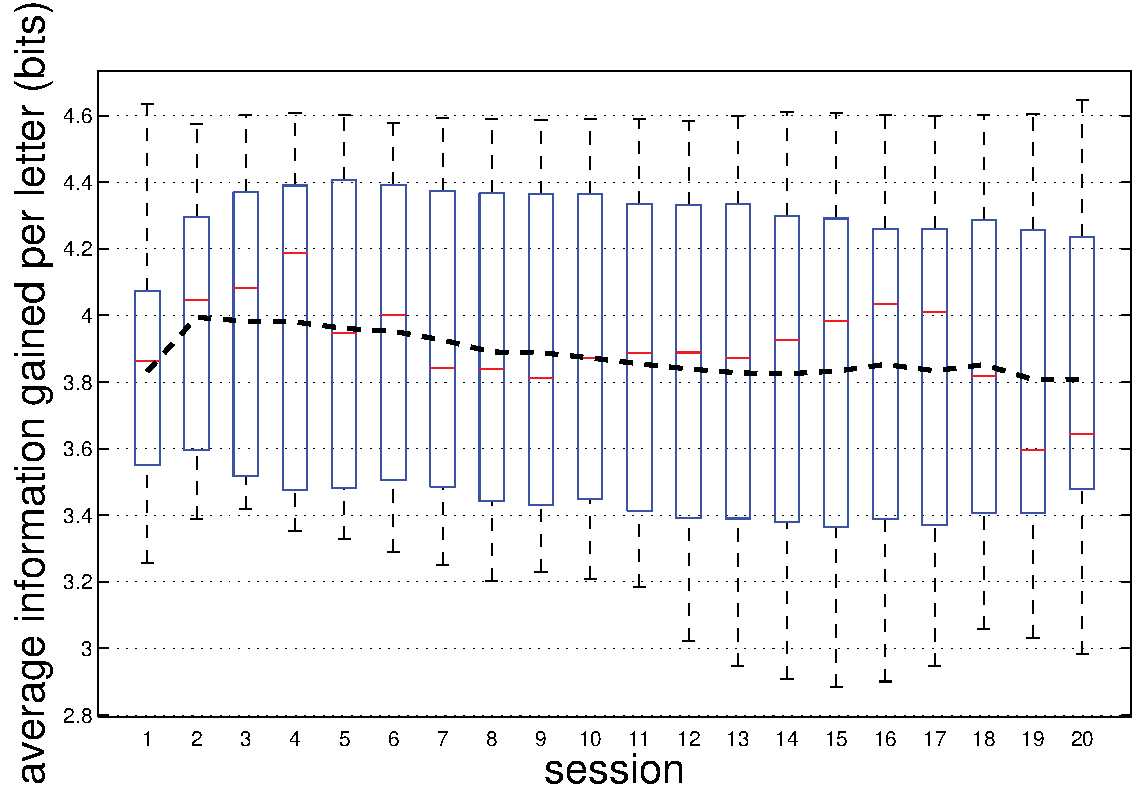
\includegraphics[width=\columnwidth]{figures/IUI_total_logloss_p_first.pdf}
    \caption{Mutual information}
    \label{fig:mutual_information}
  \end{subfigure}
  \caption{The average writing time per session and the average mutual
    information per session under the condition $\RFixed$.}
\end{figure}


In Figure~\ref{fig:channel_rate_per_user}, we compare $\RAdapt$ and
$\RFixed$ for each user. We found that the channel rate of
$\RAdapt$ is significantly higher than that of $\RFixed$ with $p <
0.0006$.  This result confirms that the computer adaptation helps
improving the overall channel rate. In addition, we calculate the
theoretical maximum of the channel rate under the assumption of the
perfect recognition, denoted by $\RIdeal$. The maximum rates are
given by $H(\predFinal) / \expectedDuration$ and we approximated $H(\predFinal) =
\log_2(26)$.

\begin{figure}
  \centering
  \begin{subfigure}[b]{\columnwidth}
    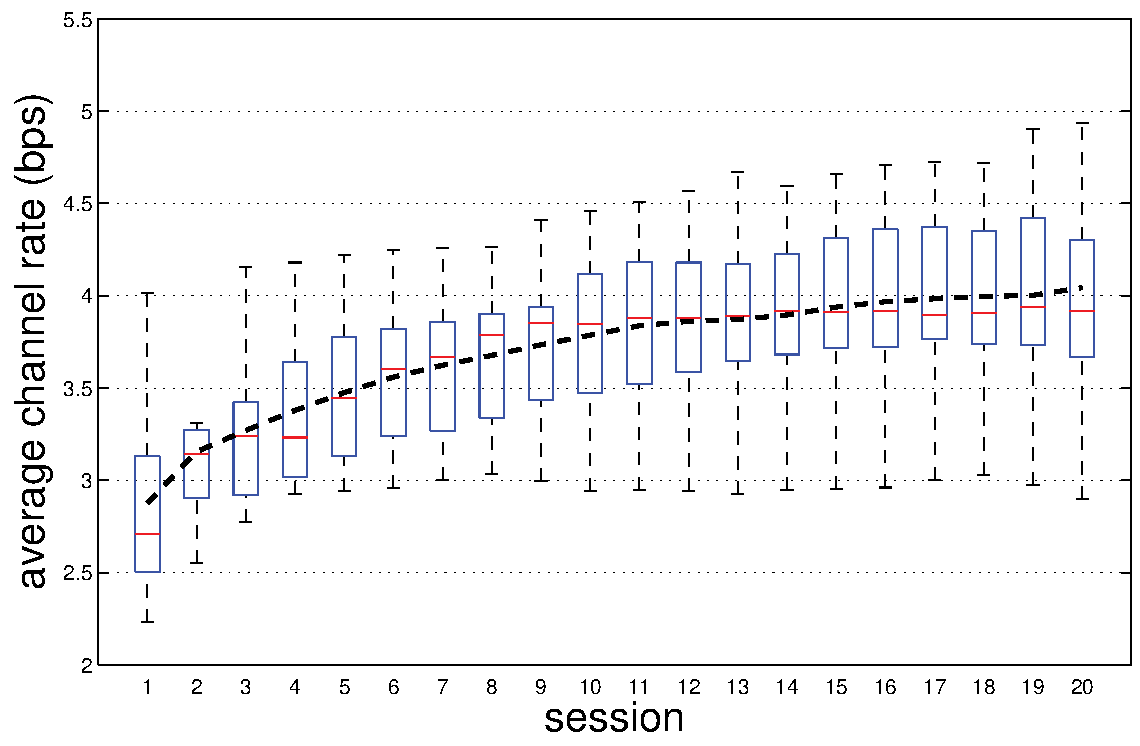
\includegraphics[width=\columnwidth]{figures/IUI_BPS_p_adapt.pdf}
    \caption{$\RAdapt$}
    \label{fig:channel_rate_adapt}
  \end{subfigure}
  \begin{subfigure}[b]{\columnwidth}
    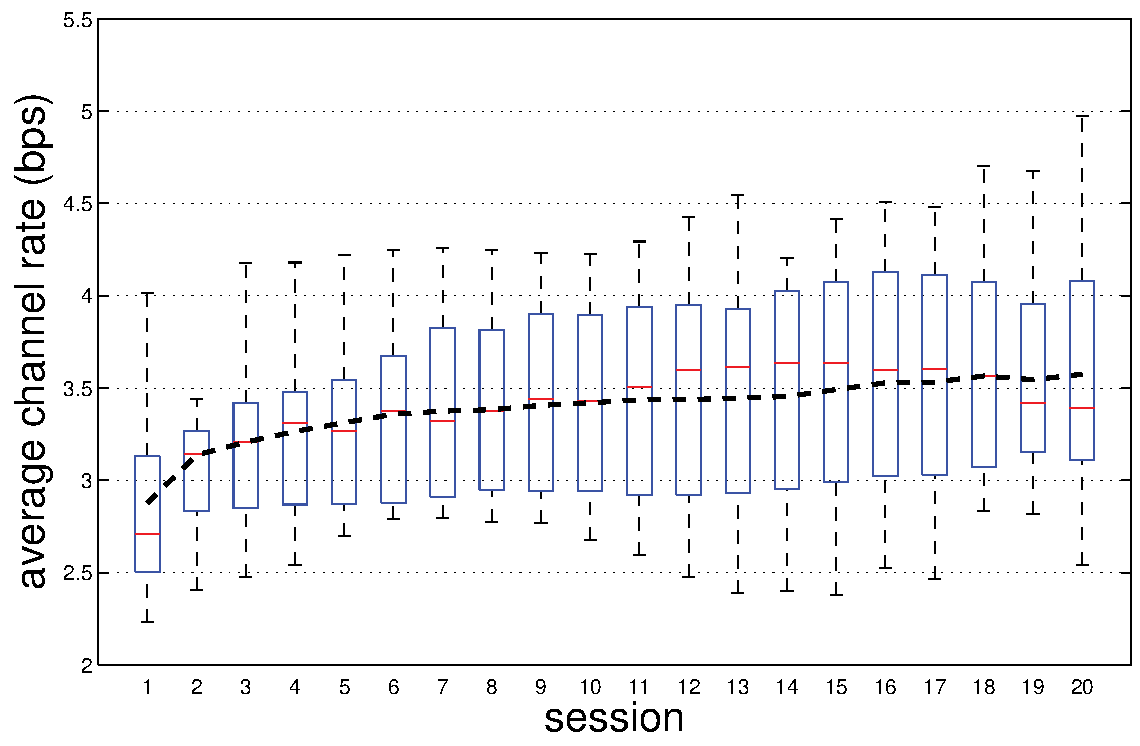
\includegraphics[width=\columnwidth]{figures/IUI_BPS_p_first.pdf}
    \caption{$\RFixed$}
    \label{fig:channel_rate_fixed}
  \end{subfigure}
  \begin{subfigure}[b]{\columnwidth}
    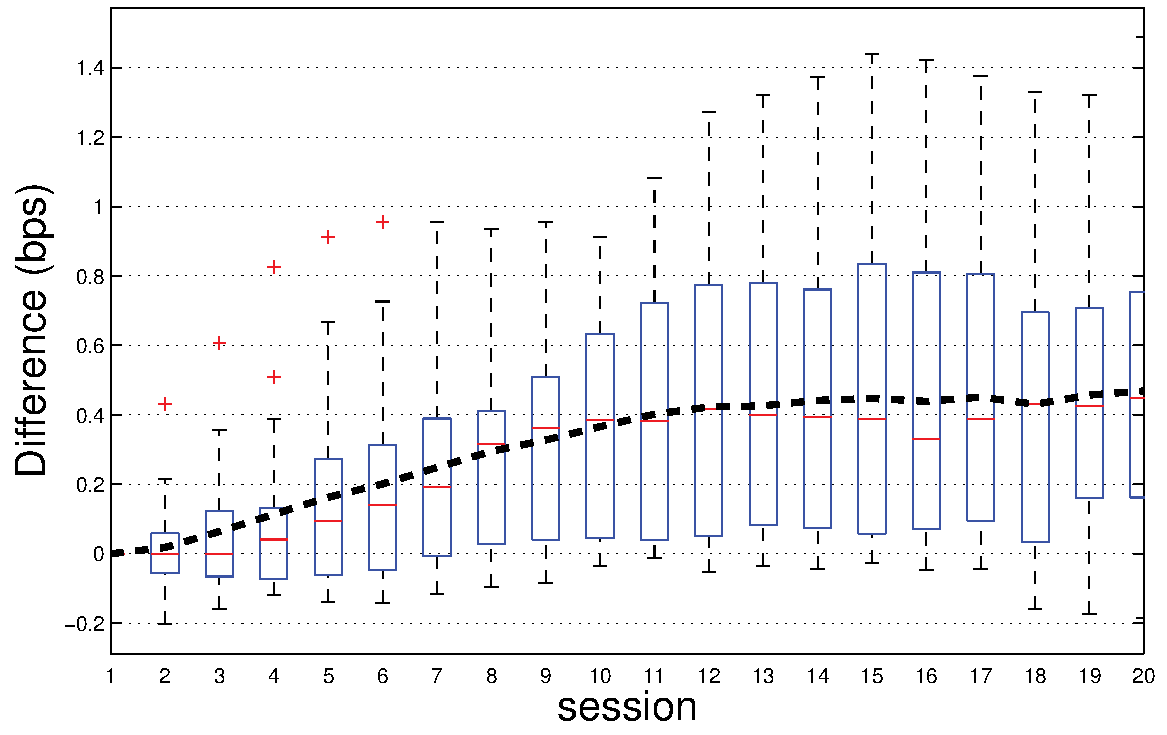
\includegraphics[width=\columnwidth]{figures/IUI_BPS_diff_p_first.pdf}
    \caption{$\RAdapt - \RFixed$}
    \label{fig:channel_rate_diff}
  \end{subfigure}
  \label{fig:channel_rate}
  \caption{Channel rate per session of each user with
    (\ref{fig:channel_rate_adapt}) and without (\ref{fig:channel_rate_fixed})
    presence of machine learning. }
\end{figure}

\begin{figure}
  \centering
  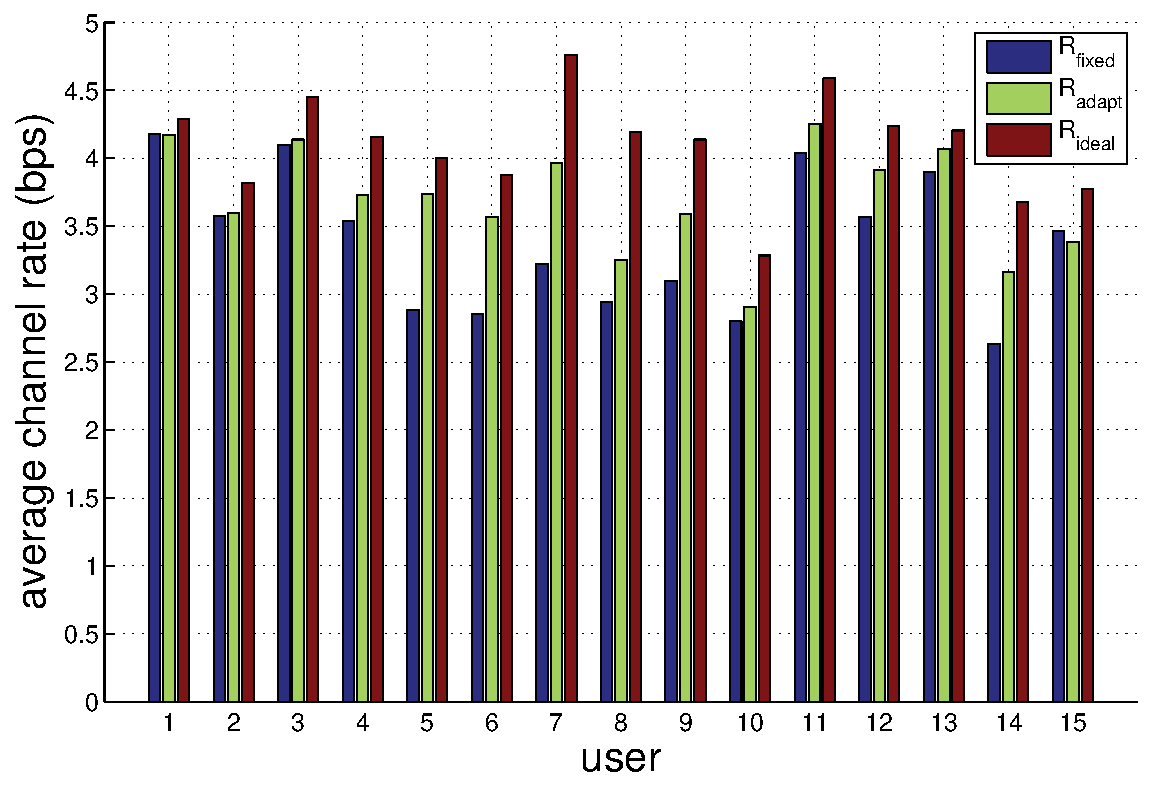
\includegraphics[width=.9\columnwidth]{figures/IUI_user_summary.pdf}   
  \caption{The average channel rate of each user in $\RAdapt$ and
    $\RFixed$. $\RIdeal$ shows the maximum channel rate possible given the
    average writing speed of each user. }
  \label{fig:channel_rate_per_user}
\end{figure}

In the case of perfect recognition, a simple way to increase the
channel rate is to increase the size of the character set
$\intentSet$. However, in reality, doing so can lead to a
recognition error rate which impairs the channel rate. An interesting
future direction is to find a character set that would maximize the channel
rate. Figure~\ref{fig:histogram_english_rate} reveals the efficiency of each
letter for our handwriting channel. Characters with complex stokes,
such as 'q', 'g','k', are not as efficient as characters with simple
strokes such as 'c' ,'o', 'l'. 

\begin{figure}
  \centering
  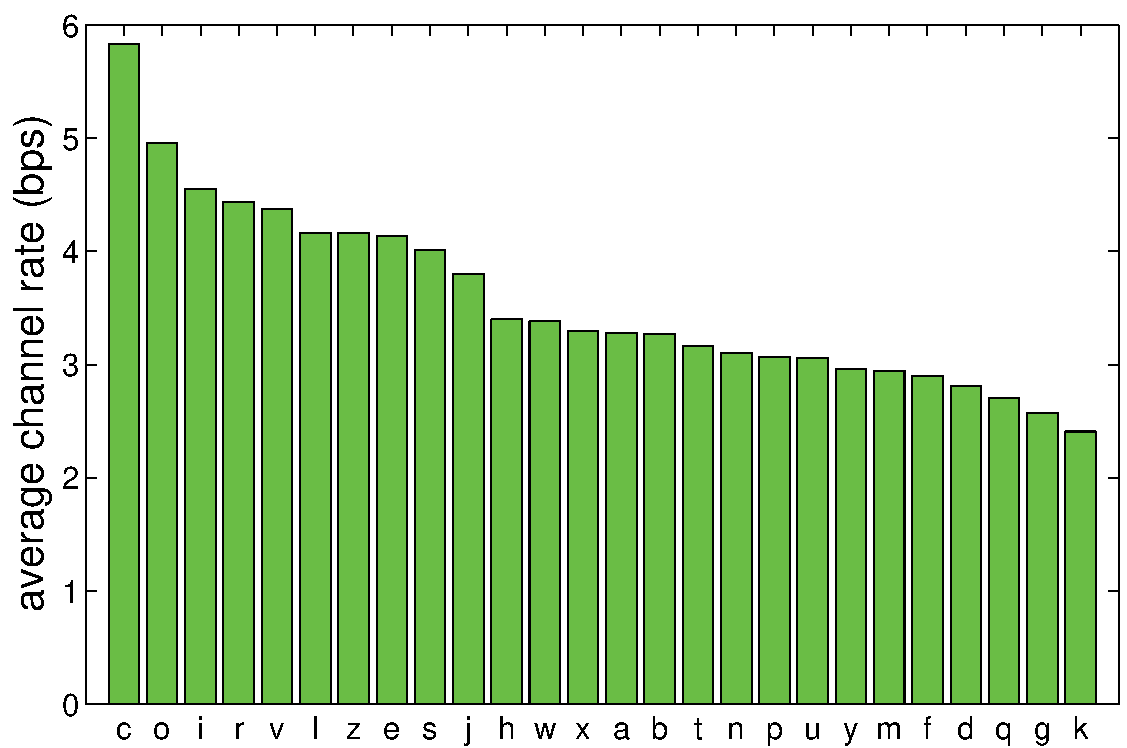
\includegraphics[width=0.9\columnwidth]{figures/histogram_channel_rate.pdf}
  \caption{Average channel rate of each character under the condition $\RAdapt$.}
  \label{fig:histogram_english_rate} 
\end{figure}


\subsection{Confusion and the conditional entropy}

In addition to the experiment, we performed a detailed analysis on the
recognition errors made by the system to visualize and understand
about the mistakes. Specifically, we computed a confusion matrix based
on the data from the experiment. The confusion matrix indicated that
99\% of the mistakes concentrate among 33 pairs of prototypes out of
the total of 2278 pairs. This suggests that the confusions only happen
between a few pairs of prototypes. Figure~\ref{fig:prototypes} shows
some of the confusion pairs and the handwritten examples that were
misrecognized. By inspection, we found that the confused handwritten
characters were very similar for some letter pairs such as 'n'-'u',
'n'-'h' or 'r'-'v'.

The confusion is closely related to the conditional entropy
$H(\predFinal | \intent)$. When this is no confusion, the entropy quickly
converges to zero as demonstrated in Figure~\ref{fig:entropy_z}. This
suggests that early termination of the writing is viable. The system
could have notified the user to stop writing at \frame{2} and it can
still recognize the partial handwriting as a 'z'. On the other hand,
when there is a confusion, the entropy does not necessarily converge
to zero when at the end of the writing e.g. the entropy of 'y' in
Figure~\ref{fig:entropy_y}.

\begin{figure*}
  \centering
  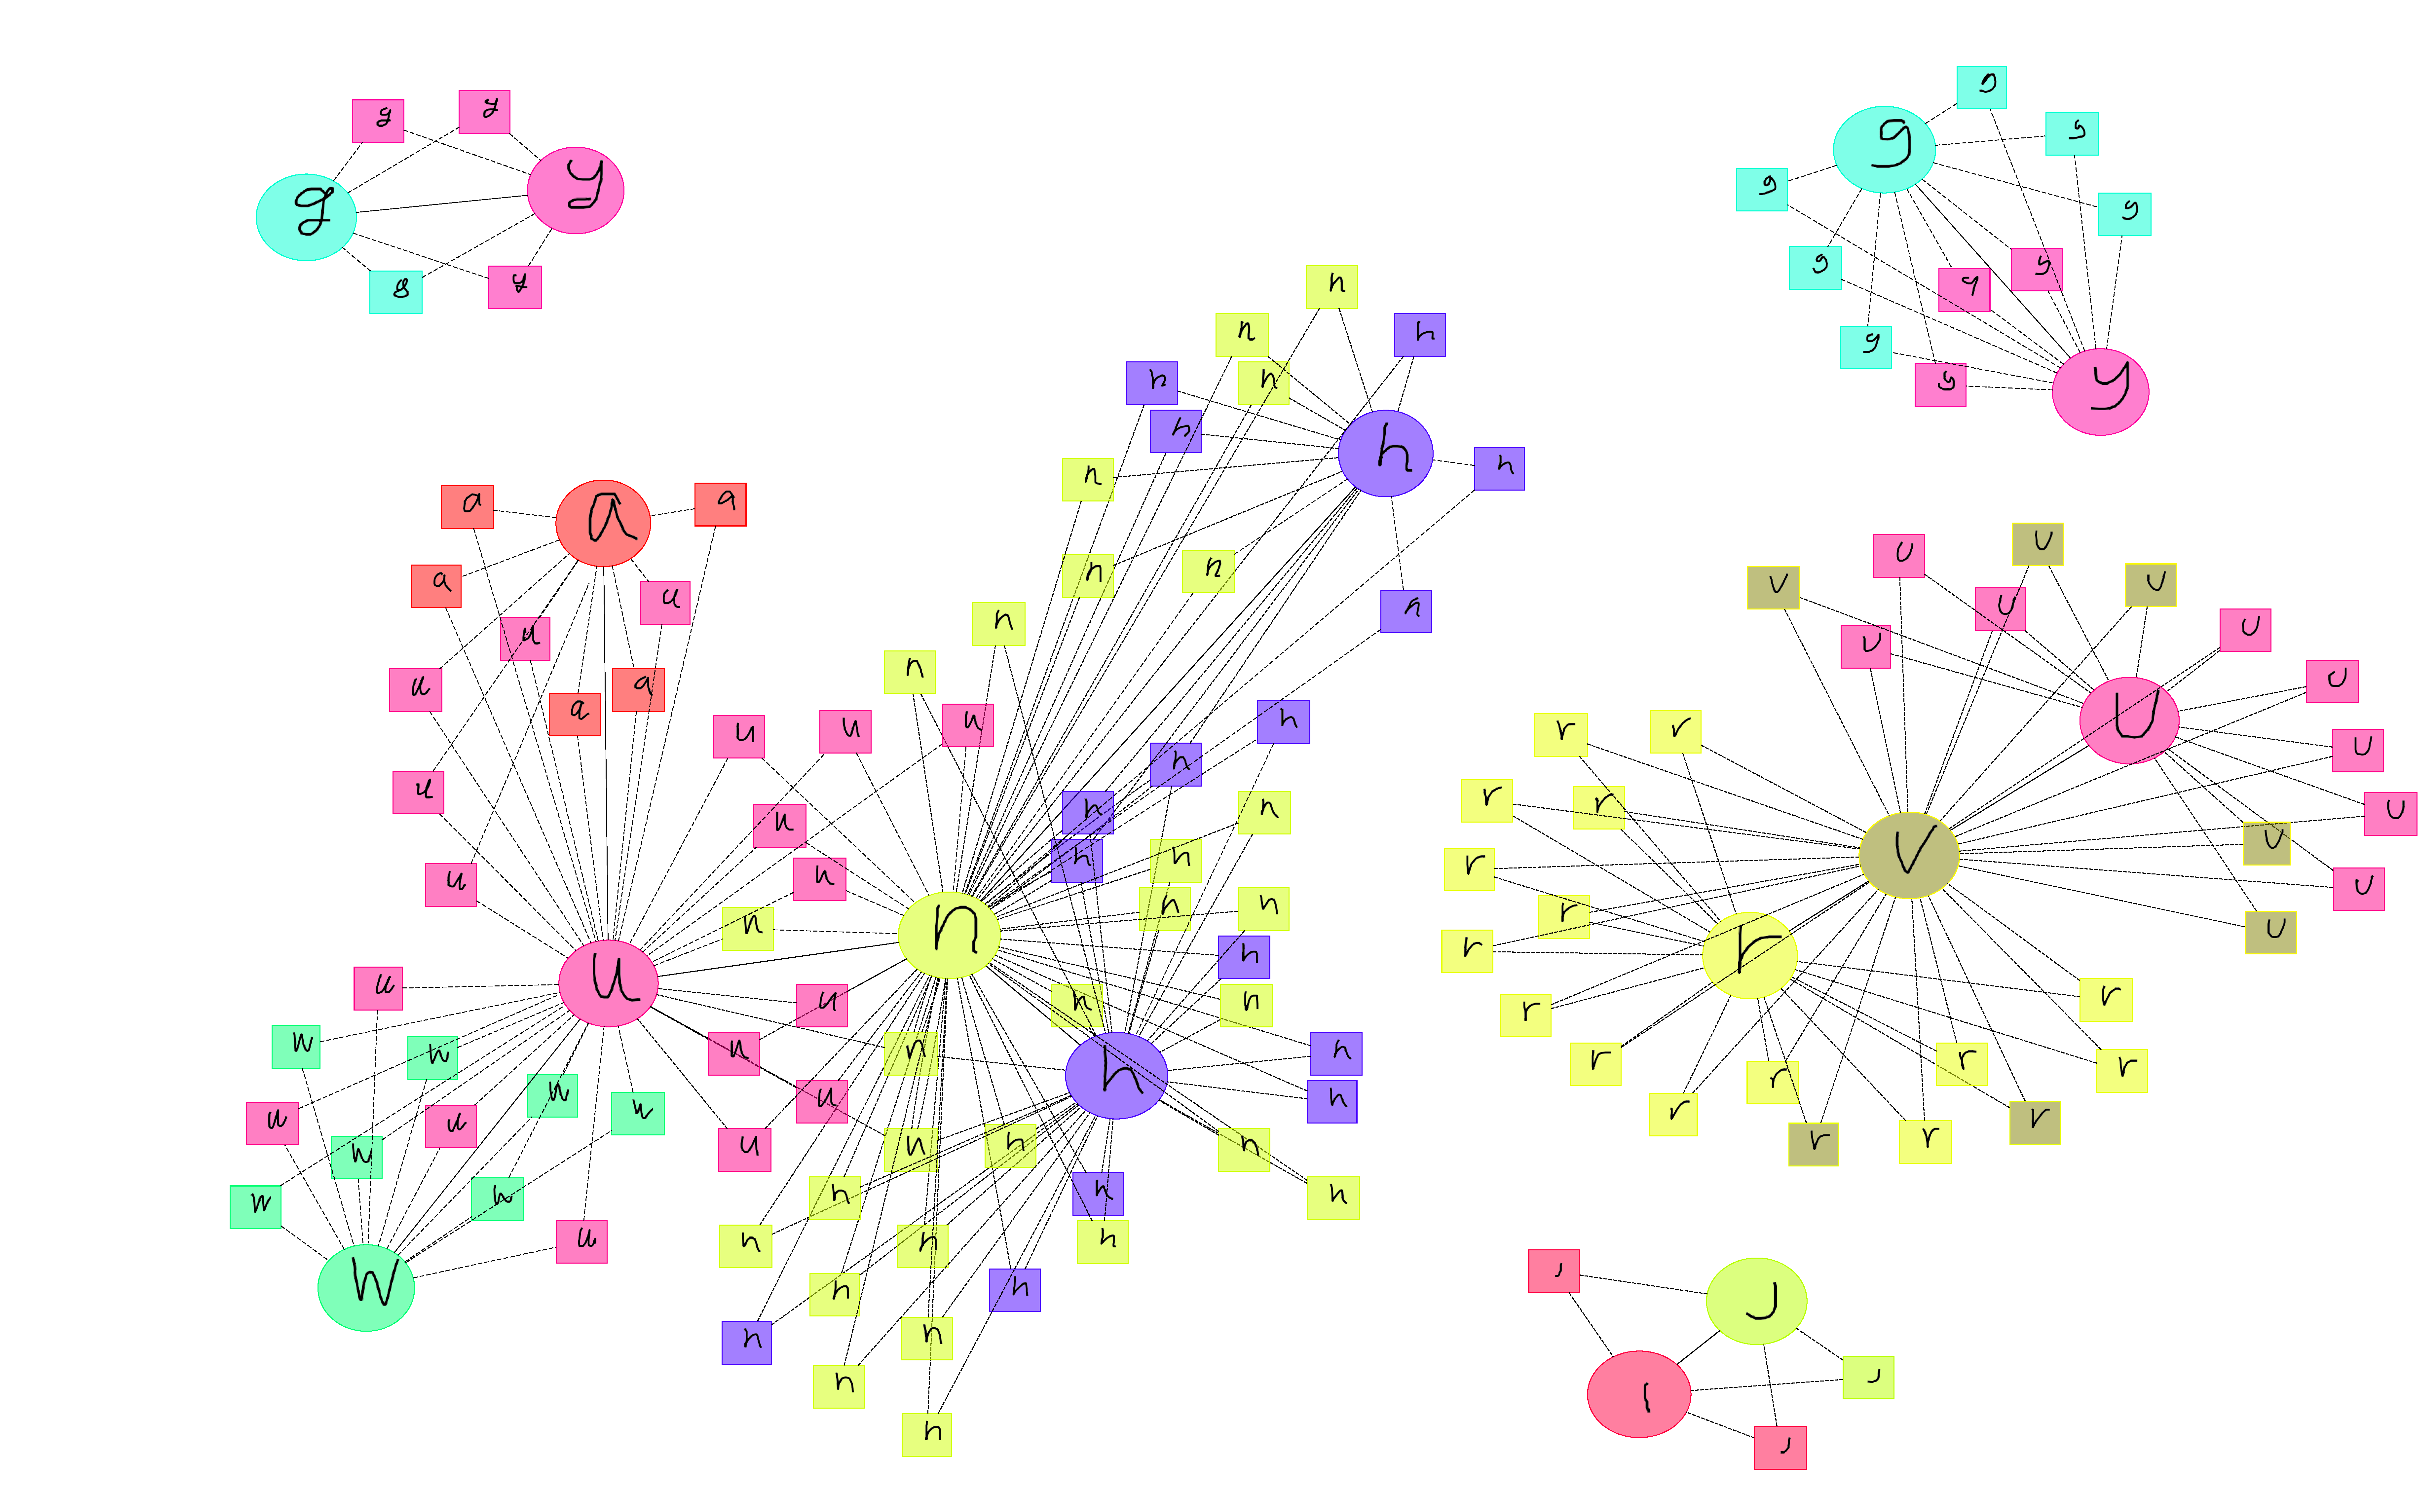
\includegraphics[width=0.9\textwidth]{figures/confusion.pdf}
  \caption{The confusion between two prototypes (circle nodes)
    is represented by an edge. Some of the confusing examples are
    shown in square nodes. Only confusable prototypes are shown. }
  \label{fig:prototypes}
\end{figure*}


In Figure~\ref{fig:entropy}, we look closely at the evolution of
$\pred{t}$ of a confusable triplet: 'g', 'y' and 'q'. In
Figure~\ref{fig:entropy_g}, the probability of 'g' starts to dominate
other contenders e.g. 's' and 'a' after \frame{3}. Similarly, in
Figure~\ref{fig:entropy_q}, the posterior distribution evolves
similarly to what we observe in Figure~\ref{fig:entropy_g} then the
probability of 'q' increases towards the end of the handwriting. This
indicates that the crucial information that distinguishes between 'g'
and 'q' is concentrated towards the end of the trajectory. Based
on~\ref{fig:prototypes}, the system sometimes confuses 'y' with 'g'. We
suspect that such confusion happens when the probability of 'y' between
\frame{1} and \frame{2} is too small relative to the probabilities of the
contenders. The posterior distribution of a correctly recognized 'y'
is shown in Figure~\ref{fig:entropy_y}.

\begin{figure*}
  \centering
  \begin{subfigure}[b]{0.35\textwidth}
    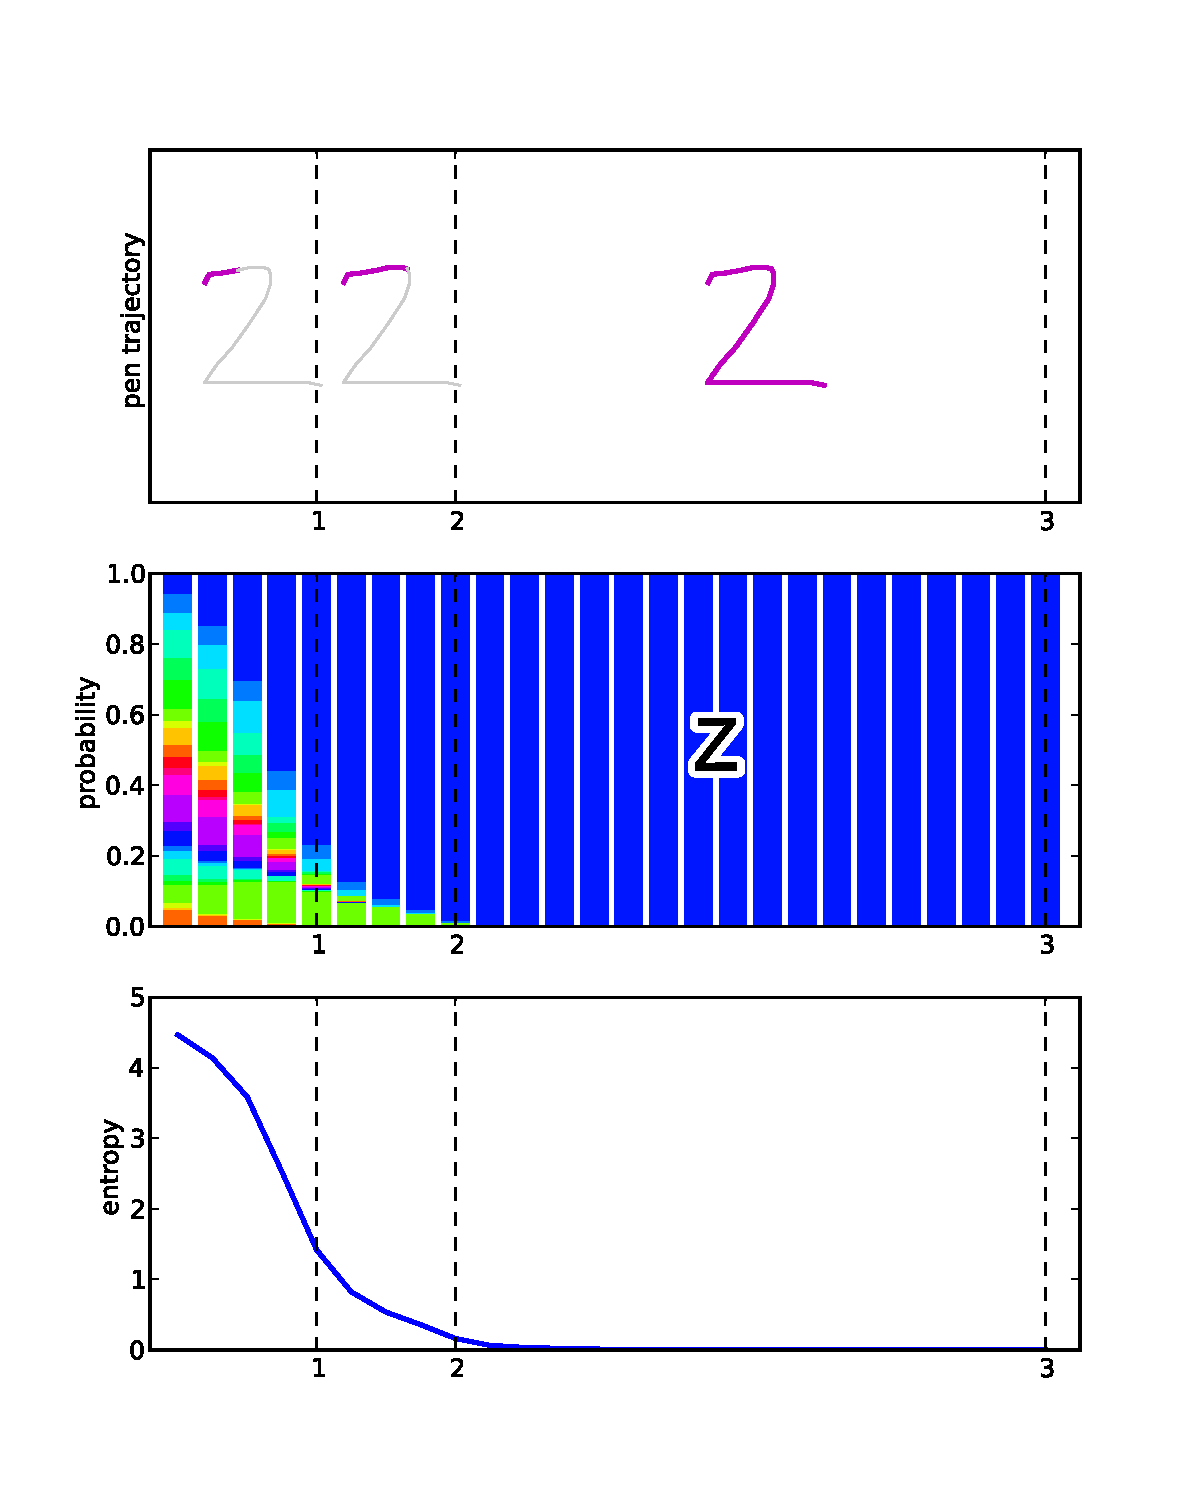
\includegraphics[width=\textwidth]{figures/entropy_z.pdf}
    \caption{}
    \label{fig:entropy_z}
  \end{subfigure}
  \begin{subfigure}[b]{0.45\textwidth}
    \begin{tabular}{c}
      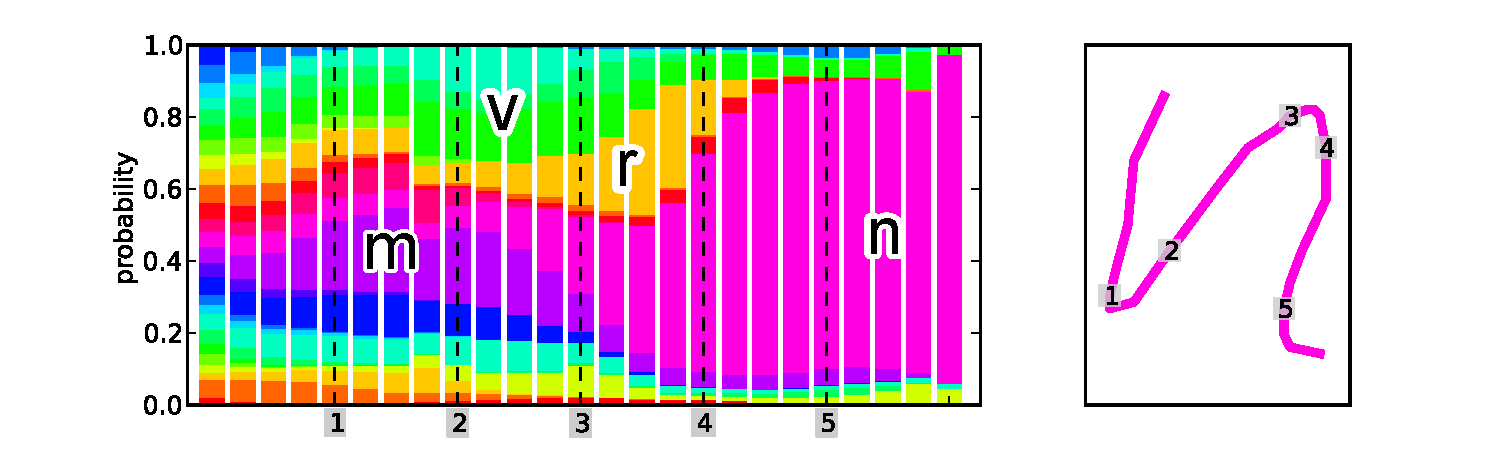
\includegraphics[width=\textwidth]{figures/best_l1.pdf}\\
      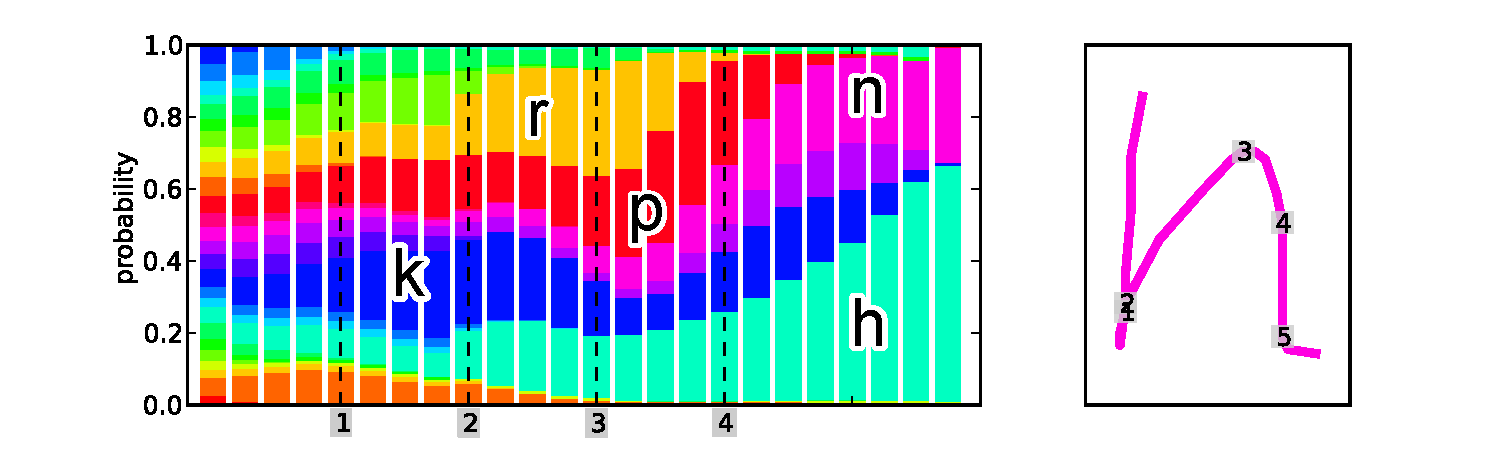
\includegraphics[width=\textwidth]{figures/unclear_l1.pdf}\\
      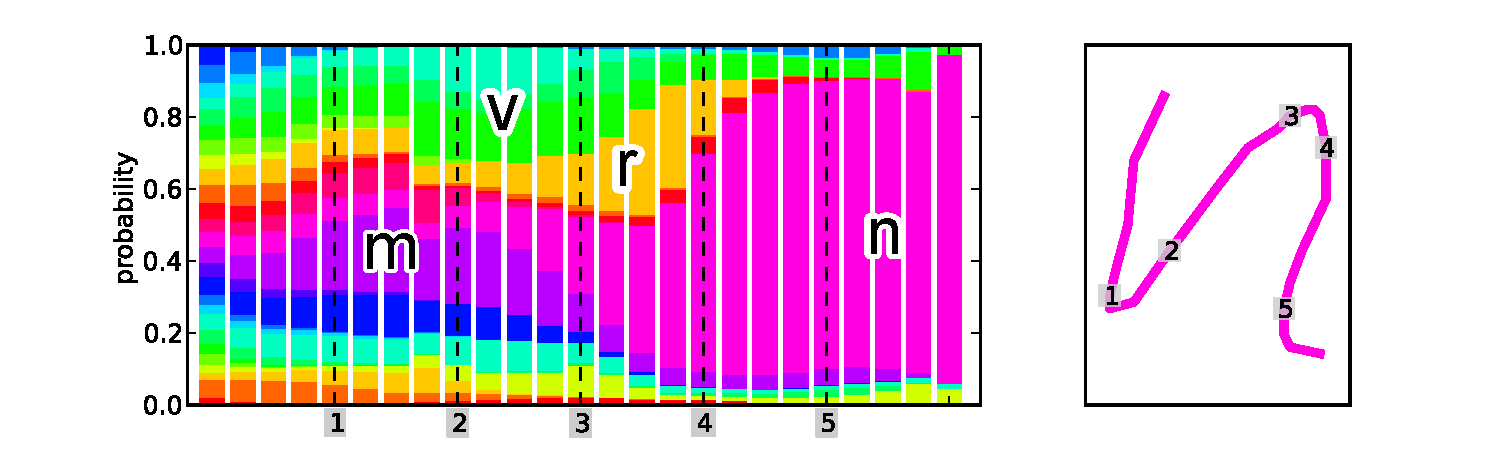
\includegraphics[width=\textwidth]{figures/best_l2.pdf}
    \end{tabular}
    \caption{}
    \label{fig:confusion}
  \end{subfigure}
  \caption{The conditional entropy $\condEntropy$ quickly reduces to 0
    when there is no confusion with other prototypes.  --- Three
    handwritten examples from a single user. The top example and the
    bottom example are recognized correctly as an 'n' and an 'h'
    respectively. The middle example is recognized as an 'h' instead
    of the true label 'n'.}
\end{figure*}

In Figure~\ref{fig:confusion}, we show the posterior distributions
over time of 3 examples selected from a single user: a correctly
recognized 'n', a correctly recognized 'h' and an 'n' that was
recognized as an 'h'. We notice that, when the system correctly
recognized an 'n', the probability of 'n' increases significantly
between \frame{2} and \frame{4}, which corresponds to the upward
movement of the hand when writing both 'n' and 'h'. This information
can be delivered to the user in a form of the instructional feedback
to encourage the user to pay more attention to the upward movement part
when writing the pair.

\begin{figure*}
  \centering
  \begin{subfigure}[b]{0.25\textwidth}
    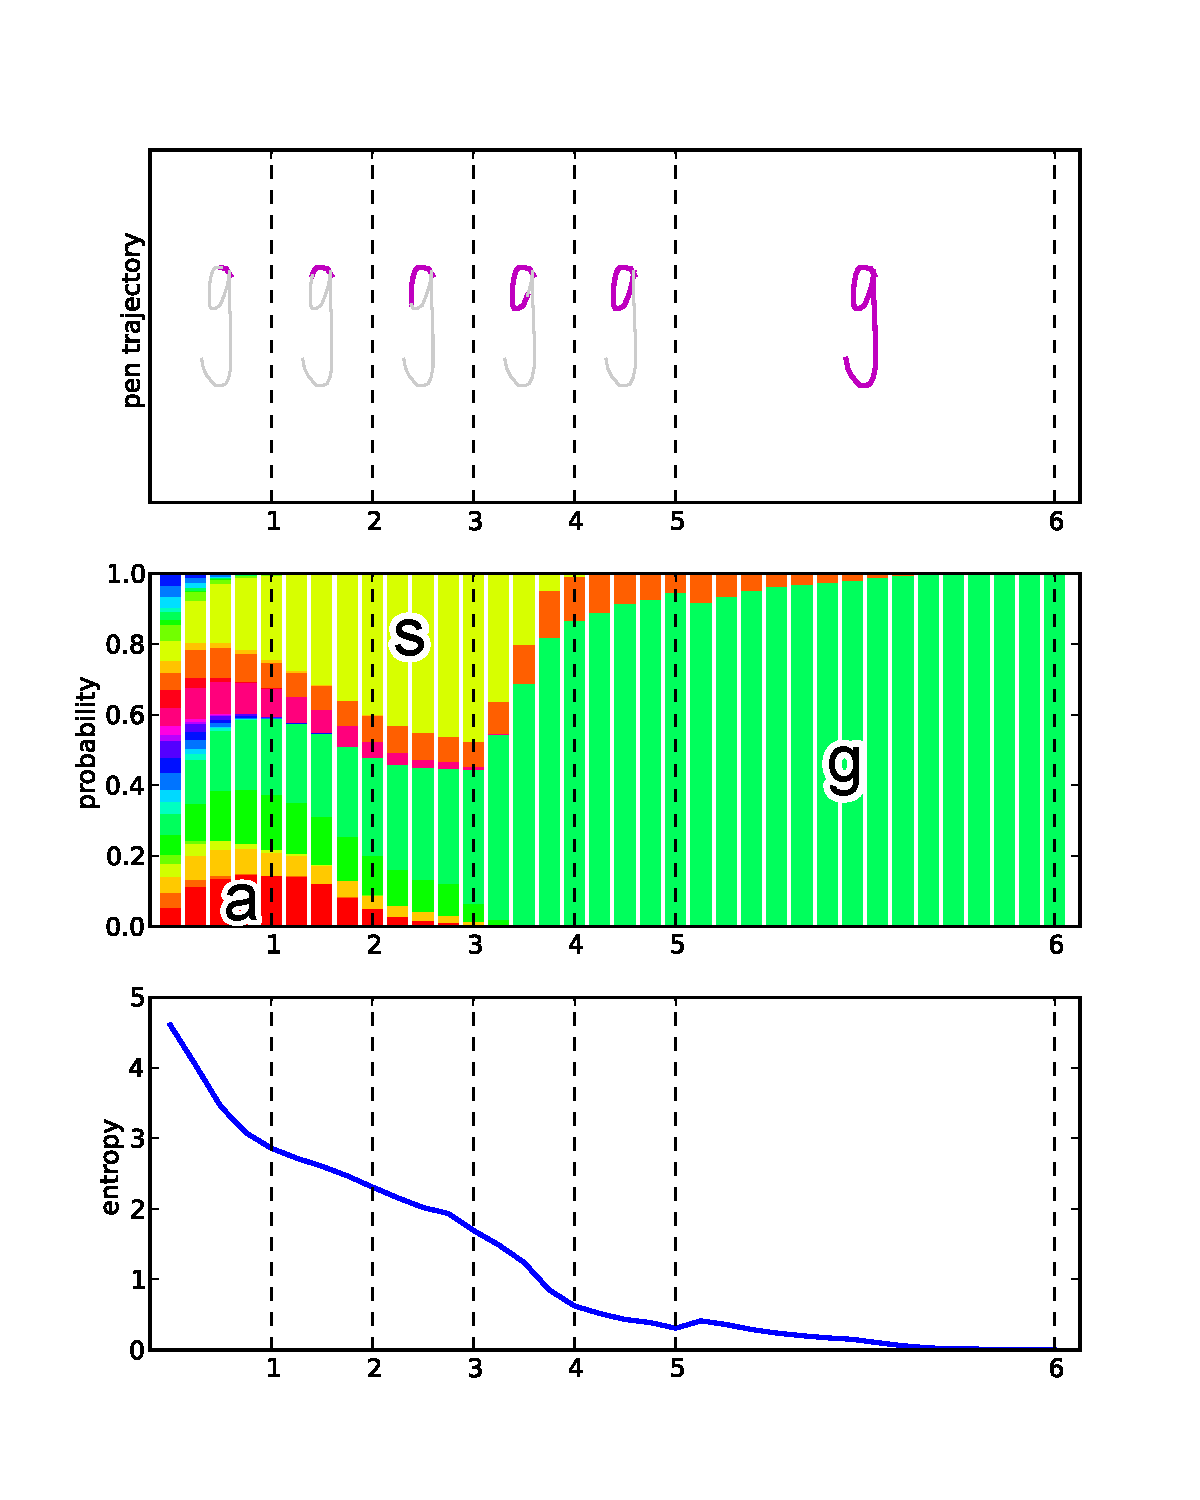
\includegraphics[width=\textwidth]{figures/entropy_g.pdf}
    \caption{}
    \label{fig:entropy_g}
  \end{subfigure}
  \begin{subfigure}[b]{0.25\textwidth}
    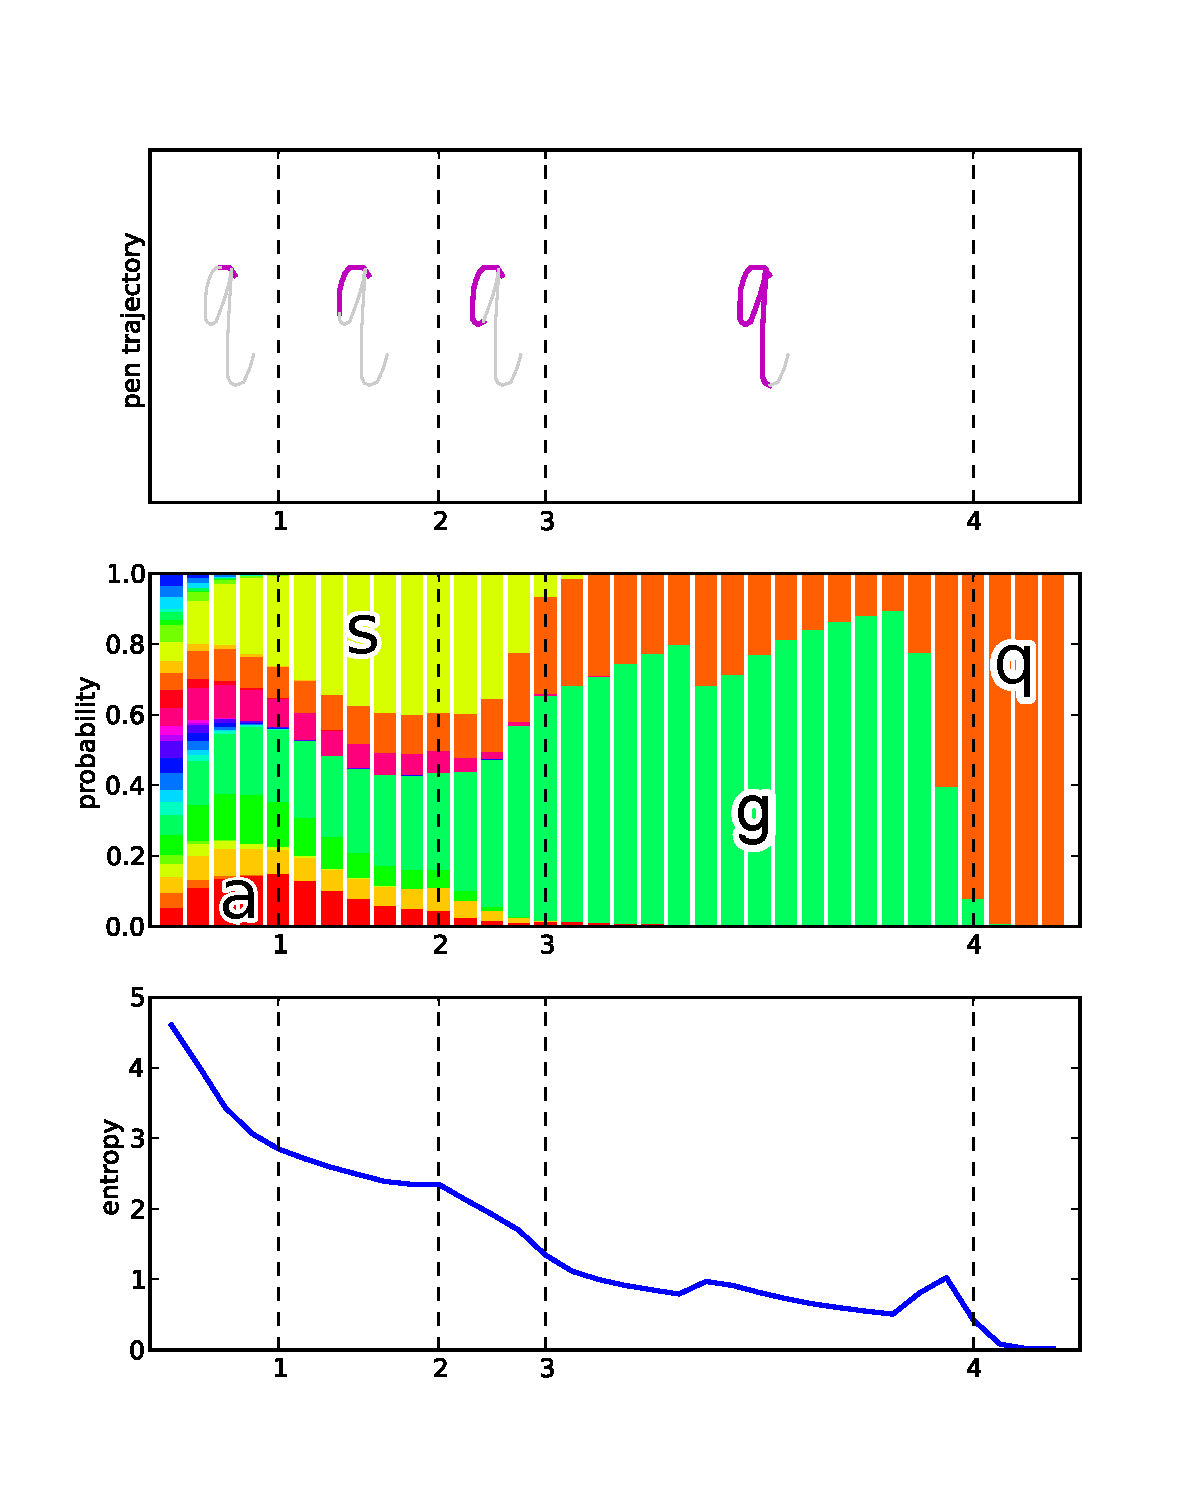
\includegraphics[width=\textwidth]{figures/entropy_q.pdf}
    \caption{}
    \label{fig:entropy_q}
  \end{subfigure}
  \begin{subfigure}[b]{0.25\textwidth}
    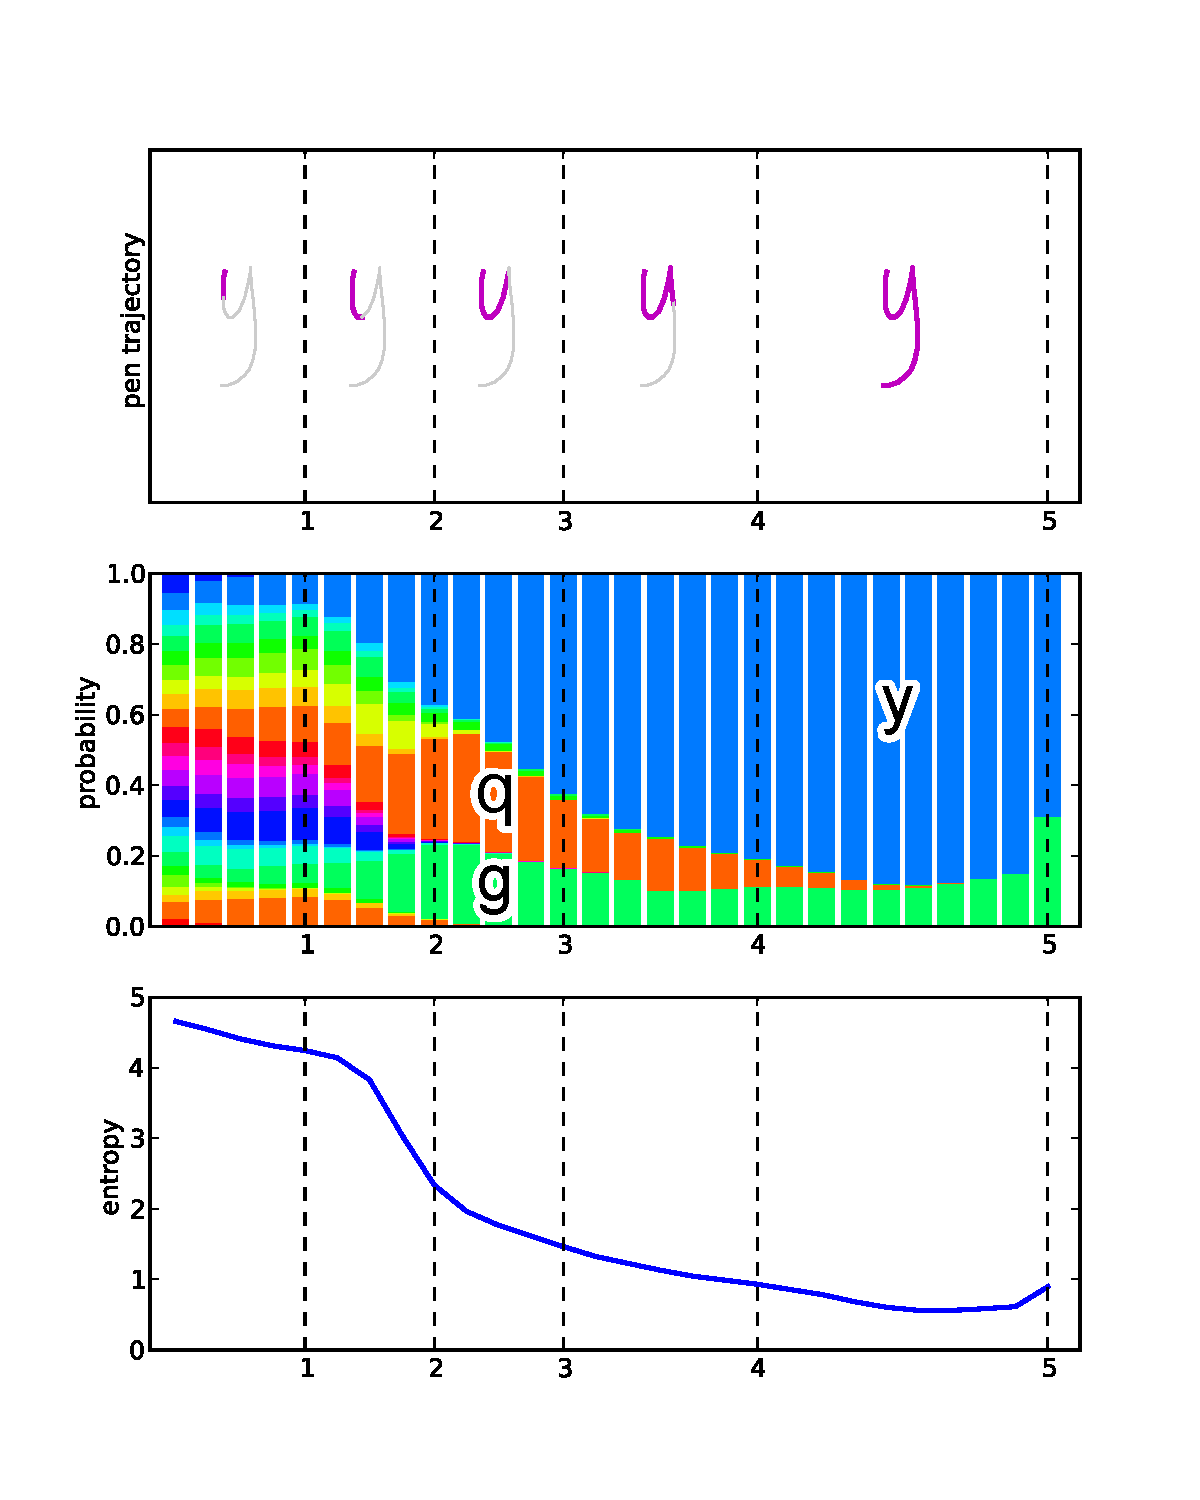
\includegraphics[width=\textwidth]{figures/entropy_y.pdf}
    \caption{}
    \label{fig:entropy_y}
  \end{subfigure}
  \caption{The posterior distributions as a function of time. The top
    row is the partial handwriting trajectories up to each dotted
    line. The middle row is the likelihood distributions over time
    where each color corresponds to each label. The bottom row is the
    entropy over time. }
  \label{fig:entropy}
\end{figure*}


\section{Conclusions}
\label{sec:conclusions}

In this paper, we presented a theoretical framework for quantifying
the data transfer rate of a system that combines a human writer and a
handwriting recognition system. We developed an adaptative character
recognition algorithm and showed the results of a small deployment of
the system. From the results, we concluded that both the adaptation of
the computer (machine learning) and the adaptation of the human
(learning to write) needs to be considered together in order to design
a system that maximizes the information rate. Finally, we performed a
detailed analysis of the information transmission within the time a
single letter is written. Based on this analysis we can pinpoint the
location where the writer is failing to clearly disambiguate two
letters. On the other hand, we find other letters which are recognized
shortly after they begin. These identify inefficiencies in the coding
process and suggests ways we can teach the user to write in a way that
would increase the over channel rate of the system.


% Balancing columns in a ref list is a bit of a pain because you
% either use a hack like flushend or balance, or manually insert
% a column break.  http://www.tex.ac.uk/cgi-bin/texfaq2html?label=balance
% multicols doesn't work because we're already in two-column mode,
% and flushend isn't awesome, so I choose balance.  See this
% for more info: http://cs.brown.edu/system/software/latex/doc/balance.pdf
%
% Note that in a perfect world balance wants to be in the first
% column of the last page.
%
% If balance doesn't work for you, you can remove that and
% hard-code a column break into the bbl file right before you
% submit:
%
% http://stackoverflow.com/questions/2149854/how-to-manually-equalize-columns-
% in-an-ieee-paper-if-using-bibtex
%
% Or, just remove \balance and give up on balancing the last page.
%
\balance

% If you want to use smaller typesetting for the reference list,
% uncomment the following line:
% \small
\bibliographystyle{acm-sigchi}
\bibliography{library}
\end{document}
